\section{计算性密码与语义安全性}

正如我们在香农定理(定理 \ref{theo:2-5})中所看到的,实现完美安全的唯一方法是拥有和消息一样长的密钥。然而这是很不现实的,我们往往希望能够用一个短的密钥(比如几百比特)来加密一个长的消息(比如几兆字节)。绕过香农定理的唯一方法是放松我们对安全性的要求。我们要做的是,不考虑所有可能的对手,而只考虑\emph{计算上可行}的对手,也就是说,``真实世界"对手必须在真实的计算机上使用合理的时间和内存进行计算。这就将我们导向了一个稍弱的安全定义,称为\textbf{语义安全(semantic security)}。这个安全定义更加灵活,只要一个允许变长消息空间的密码不向对手泄露\emph{除消息长度之外的}任何有用信息,我们就称该密码是安全的。另外,由于我们现在关注的是``实用性"而不是``数学上的可能性",我们还会坚持认为,加密和解密函数本身都是有效算法,而不是任意的函数。

\subsection{计算性密码的定义}\label{subsec:2-2-1}

一个\textbf{计算性密码(computational cipher)} $\mathcal{E}=(E,D)$ 是一对有效密码算法 $E$ 和 $D$。加密算法 $E$ 接受一个密钥 $k$ 和一条消息 $m$ 作为输入,生成并输出一条密文 $c$。揭秘算法$D$接受一个密钥$k$和一条密文$c$作为输入,并输出一条消息$m$。密钥 $k$ 位于某个有限的密钥空间 $\mathcal{K}$ 中,消息 $m$ 位于某个有限的消息空间 $\mathcal{M}$ 中,密文 $c$ 位于某个有限的密文空间 $\mathcal{C}$ 中。正如香农密码一样,我们称 $\mathcal{E}$ 定义在 $(\mathcal{K},\mathcal{M},\mathcal{C})$ 上。

尽管对于我们在本章中的目的来说,这并不是必要的,但我们仍将允许加密函数 $E$ 是一种概率性算法(参见第\ref{chap:apdx-4}章)。这意味着对于固定的输入 $k$ 和 $m$,$E(k,m)$ 的输出值可能是多个值中的一个。为了强调这种计算的概率性质,我们用:
$$
c\overset{\rm R}\leftarrow E(k,m)
$$
来表示执行$E(k,m)$并将其输出分配给程序变量$c$的过程。在本书中,只要我们使用概率性算法,我们就会使用这一符号。同样地,我们用:
$$
k\overset{\rm R}\leftarrow\mathcal{K}
$$
来表示从密钥空间 $\mathcal{K}$ 中随机均匀地选取一个值赋给程序变量$k$的过程。我们会使用类似的符号表示从任何有限集中均匀随机抽样的过程。

在本章中,我们不会介绍任何具体地概率加密算法(我们将在第\ref{chap:5}章中看到这方面的第一个例子)。虽然我们也可以令解密算法也是概率性的,但是并没有这个必要,因此我们只会讨论使用确定性解密算法的密码。然而,我们允许解密算法返回一个(与所有有效消息都不同的)特殊的$\mathsf{reject}$,这在某些场合是很有用的,可以表明解密过程中发生了某种错误。

由于加密算法是概率性的,对于一个给定的密钥 $k$ 和消息 $m$,加密算法可能会输出许多可能的密文之一;然而,这些可能的密文中的每一个都应该解密为 $m$。我们可以更正式地表述这个\textbf{正确性要求}:对于所有的密钥 $k\in\mathcal{K}$ 和消息 $m\in\mathcal{M}$,如果我们执行:
$$
c\overset{\rm R}\leftarrow E(k,m),\;\;
m'\overset{\rm R}\leftarrow D(k,c)
$$
那么 $m=m'$ 成立的概率为 $1$。


\begin{quote}
\begin{tcolorbox}[colframe=black,colback=white,boxrule=0.6pt,arc=0pt]
\emph{从现在开始,每当我们提到一个\textbf{密码}时,我们指的都是如上所定义的\textbf{计算性密码}。此外,如果加密算法恰好也是确定性的,那么我们就可以称该密码为一个\textbf{确定性密码}。}
\end{tcolorbox}
\end{quote}

请注意,任何确定性密码都是香农密码,但是计算性密码不一定是香农密码(如果其有一个概率性加密算法),香农密码也不一定是计算性密码(如果其加密或解密操作没有有效实现)。

\begin{example}
一次性密码本(见例 \ref{exmp:2-1})和变长一次性密码本(见例 \ref{exmp:2-2})都是确定性密码,因为它们的加密和解密操作都可以通过有效的确定性算法来实现。替换密码(见例 \ref{exmp:2-3})只要字母表 $\Sigma$ 不是太大,也属于确定性密码。事实上,在显而易见的实现方法中,一个密钥也就是对$\Sigma$的一种置换方案,会用一个以$\Sigma$为索引的数组来表示,所以我们需要$O(|\Sigma|)$的空间来存储一个密钥。因此,这只适合大小合理的$\Sigma$的情形。例 \ref{exmp:2-4} 中讨论的加性一次性密码本也是一个确定性密码,因为加密和解密操作都可以有效地实现(如果$n$很大,可能需要特殊的软件来进行大整数的算术运算)。
\end{example}

\subsection{语义安全性的定义}

为了引入语义安全性的定义,考虑一个定义在 $(\mathcal{K},\mathcal{M},\mathcal{C})$ 上的确定性密码 $\mathcal{E}=(E,D)$。我们重新考察定理 \ref{theo:2-3} 给出的关于完美安全性的表述。它表明,对于密文空间上所有的谓词逻辑 $\phi$ 和所有消息 $m_0$,$m_1$,我们都有:
\begin{equation}\label{eq:2-3}
\Pr[\phi(E(\mathsf{k},m_0))]=\Pr[\phi(E(\mathsf{k}, m_1))]
\end{equation}
其中 $\mathsf{k}$ 是一个在 $\mathcal{K}$ 上均匀分布的随机变量。现在,我们不再要求概率相等,而只是要求它们非常接近,即:
\begin{equation}\label{eq:2-4}
|\Pr[\phi(E(\mathsf{k},m_0))]-\Pr[\phi(E(\mathsf{k}, m_1))]|\leq \epsilon
\end{equation}
对一个非常小的,或者\emph{可以忽略不计}的$\epsilon$成立。就其本身而言,这种放松并没有多大帮助(见练习 2.5)。然而,我们现在不再要求式 \ref{eq:2-4} 对所有可能的谓词 $\phi$ 和消息 $m_0$,$m_1$ 都成立,而是只要求式 \ref{eq:2-4} 对所有可以由某种有效算法生成的消息 $m_0$,$m_1$,以及所有可以由某种有效算法计算的谓词 $\phi$ 成立(这些有效算法可以是概率性的)。例如,假设使用最好的算法来生成$m_0$和$m_1$,以及测试一些谓词$\phi$,并使用(例如)一万台计算机在并行计算十年的情况下式 \ref{eq:2-4} 在 $\epsilon = 2^{-100}$ 的情况下仍然成立。虽然这种密码仍然不是完美安全的,但是我们可以认为这种密码对于\emph{所有的实际目的都是足够安全的}。

此外,在定义语义安全时,我们还解决了例 \ref{exmp:2-5} 中的一个问题。在那个例子中,我们看到变长一次性密码本并不满足完美安全性的定义。然而,我们希望我们的定义有足够的灵活性,以便像变长一次性密码本这样的密码,它除了长度之外不会泄露任何关于消息的信息,也可以被认为是安全的。

现在说说细节。为了精确定义语义安全性,我们将描述一个在两方之间进行的\textbf{攻击游戏(attack game)},这两方分别为\textbf{挑战者(challenger)}和\textbf{对手(adversary)}。正如我们将要看到的,挑战者会遵循一个非常简单且固定的协议。然而对手 $\mathcal{A}$ 可以遵循一个任意的(但仍然有效的)协议。挑战者和对手 $\mathcal{A}$ 按照他们各自的协议来回发送消息,在游戏结束时,$\mathcal{A}$ 将输出一些数值。事实上,我们用于定义语义安全的攻击游戏包括两个可供选择的``子游戏"或``子实验",在这两个实验中,对手会遵循相同的协议,但挑战者的行为在这两个实验中略有不同。攻击游戏还定义了一个概率空间,而这反过来又定义了对手的\emph{优势},它衡量的是在这个概率空间中两个事件的概率之差。

\begin{game}[语义安全性]\label{game:2-1}
给定一个定义在 $(\mathcal{K},\mathcal{M},\mathcal{C})$ 上的确定性密码 $\mathcal{E}=(E,D)$,对于一个给定对手 $\mathcal{A}$,我们定义两个实验:实验$0$和实验$1$。对于 $b=0,1$,我们定义:

\noindent\textbf{实验$b$:}
\begin{itemize}
	\item 对手计算长度相同的消息两个 $m_0,m_1\in\mathcal{M}$,并将其发送给挑战者。
	\item 挑战者计算 $k\overset{\rm R}\leftarrow\mathcal{K}$,$c\overset{\rm R}\leftarrow E(k,m_b)$,并将 $c$ 发送给对手。
	\item 对手输出一个比特 $\hat b\in\{0,1\}$。
\end{itemize}

对于 $b=0,1$,令 $W_b$ 为 $\mathcal{A}$ 在实验 $b$ 中输出 $1$ 的事件。那么我们将对手 $\mathcal{A}$ 相对于 $\mathcal{E}$ 的\textbf{语义安全优势}定义为:
$$
{\rm SS\mathsf{adv}}[\mathcal{A},\mathcal{E}]=|\Pr[W_0] -\Pr[W_1]|
$$
\end{game}

请注意,在上述游戏中,事件 $W_0$ 和 $W_1$ 的定义依赖于 $k$ 的随机选择、加密算法的随机选择(如果有的话)和对手的随机选择(如果有的话)所共同决定的概率空间。${\rm SS\mathsf{adv}}[\mathcal{A},\mathcal{E}]$ 的值是一个介于 $0$ 和 $1$ 之间的数字。

攻击游戏 \ref{game:2-1} 的示意图见图 \ref{fig:2-1}。如图所示,$\mathcal{A}$的``输出"实际上只是给挑战者的一个最终消息。

\begin{figure}
  \centering
  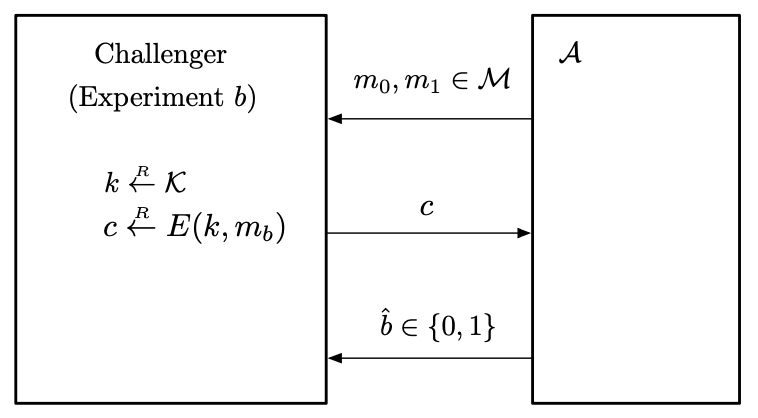
\includegraphics[width=0.5\linewidth]{figures/chapter2/fig1.png}
  \caption{攻击游戏 \ref{game:2-1} 中的实验 $b$}
  \label{fig:2-1}
\end{figure}

\begin{definition}[语义安全性]\label{def:2-2}
如果对于所有有效对手 $\mathcal{A}$,${\rm SS\mathsf{adv}}[\mathcal{A},\mathcal{E}]$ 的值都可以忽略不计,我们就称密码 $\mathcal{E}$ 是\textbf{语义安全}的。
\end{definition}

作为一个正式的定义,这还不是很完整,因为我们还没有定义``相同长度的消息"、``有效对手"和``可忽略不计"是什么意思。我们很快就会回到这个问题上。

让我们把这个正式定义与前面的讨论联系起来。假设攻击游戏 \ref{game:2-1} 中的对手 $\mathcal{A}$ 是确定性的。首先,对手以一种确定性的方式计算出消息 $m_0$和$m_1$,然后考察密文 $c$ 上的谓词 $\phi$,如果结果为真就输出 $1$,为假则输出 $0$。语义安全的意思是,式 \ref{eq:2-4} 中的 $\epsilon$ 是可以忽略不计的。如果 $\mathcal{A}$ 是概率性的,我们可以将 $\mathcal{A}$ 看作是这样的结构:他从某个适当的集合中生成一个随机数 $r$,并确定性地计算取决于$r$的消息 $m^{(r)}_0$ 和 $m^{(r)}_1$,接着评估谓词 $\phi^{(r)}$,它也取决于 $r$。这里,语义安全说明,当用 $m^{(r)}_0$、$m^{(r)}_1$ 和 $\phi^{(r)}$ 替换式 \ref{eq:2-4} 中的 $m_0$、$m_1$ 和 $\phi$ 时,$\epsilon$ 的大小仍然是可以忽略不计的,但现在的概率是针对一个随机选择的密钥和随机选择的 $r$ 值而言的。

\begin{remark}
现在让我们说一下,为什么我们要求在攻击游戏 \ref{game:2-1} 中,对手 $\mathcal{A}$ 计算出来的消息 $m_0$ 和 $m_1$ 必须是相同长度的。
\begin{itemize}
	\item 首先,消息的``长度"概念是针对特定的消息空间 $\mathcal{M}$ 而言的。换句话说,在指定一个消息空间时,我们必须指定一个规则,它能将长度(一个非负整数)与任何给定的消息关联起来。对于大多数具体的消息空间来说,这种联系是很显然的。例如,对于消息空间 $\{0, 1\}^{\leq L}$ (如例 \ref{exmp:2-2})来说,消息 $m\in\{0, 1\}^{\leq L}$ 的长度就是它的比特位数 $|m|$。然而,为了使我们的定义具有一定的普遍性,我们把长度的概念作为一个抽象概念。事实上,有些消息空间可能没有特别的长度概念,在这种情况下,所有的消息都可以被看作是长度为 $0$ 的。
	\item 其次,要求 $m_0$ 和 $m_1$ 具有相同的长度,意味着对手不会因为能够有效地根据长度区分两条密文就被认为是破坏了系统。这就是我们的正式定义所捕捉到的概念,即消息的加密被允许泄露消息的长度(但不会泄露其他信息)。
		
	我们在例 \ref{exmp:2-5} 中已经讨论过,在某些应用中,泄露消息的长度可能会带来灾难性的后果。然而,由于这个问题没有通用的解决方案,大多数现实世界的加密方案(例如TLS)根本没有尝试去隐藏消息的长度。这可能会导致真正的攻击。例如,Chen 等人表明,加密消息的长度可以揭示用户提供给云应用程序的私人数据的大量信息。他们以一个在线报税系统为例,但也有其他工作表明这种类型的攻击同样适用于很多其他的系统。
\end{itemize}
\end{remark}

\begin{example}\label{exmp:2-9}
令 $\mathcal{E}$ 是一个确定性密码,且是完美安全的。那么很容易看出,对于任意对手 $\mathcal{A}$(无论是否有效),我们都有 ${\rm SS\mathsf{adv}}[\mathcal{A},\mathcal{E}]=0$。这几乎可以立即从定理 \ref{theo:2-3} 中得出(唯一稍微复杂的是,我们在攻击游戏 \ref{game:2-1} 中的对手 $\mathcal{A}$ 可能是概率性的,但这很容易处理)。特别是,$\mathcal{E}$ 是语义安全的。因此,如果 $\mathcal{E}$ 是一次性密码本(见例 \ref{exmp:2-1}),那么对于所有对手 $\mathcal{A}$,我们有 ${\rm SS\mathsf{adv}}[\mathcal{A},\mathcal{E}]=0$,因此一次性密码本是语义安全的。由于语义安全的定义对于变长的消息空间来说是比较宽容的,所以也很容易看出,如果$\mathcal{E}$是变长一次性密码本(见例 \ref{exmp:2-2}),那么对于所有对手 $\mathcal{A}$,${\rm SS\mathsf{adv}}[\mathcal{A},\mathcal{E}]=0$都成立,因此变长一次性密码本也是语义安全的。
\end{example}

关于``有效"和``可忽略不计"这两个词,我们还要多说几句。在下面的 \ref{sec:2-3} 节中,我们将填补其余的细节(这些细节可能会稍显乏味,而且实际上并不是很有启发性)。 直观地说,\emph{可忽略不计}的意思是小到``对所有实际用途来说都是零":想像一下 $2^{-100}$ 这样的数字,如果你在下一年自燃的概率是 $2^{-100}$,那么你就不会担心这种事件的发生。我们还使用下列术语:
\begin{itemize}
	\item 一个\emph{有效对手}是一个能在``合理"时间内运行的对手。
	\item 如果 ${1}/{N}$ 可以忽略不计,就称$N$是\emph{超多项式(super-poly)}的。
	\item 一个\emph{多项式边界(poly-bounded)}的值是一个``合理"大小的数字。特别地,我们可以说,一个有效对手的运行时间是多项式边界的。
\end{itemize}

\begin{fact}\label{fact:2-6}
如果 $\epsilon$ 和 $\epsilon'$ 是两个可以忽略不计的值,而 $Q$ 和 $Q'$ 是两个多项式边界的值,那么:
\begin{enumerate}[(i)]
	\item $\epsilon+\epsilon'$ 是一个可以忽略不计的值,
	\item $Q + Q'$ 和 $Q\cdot Q'$ 都是多项式边界的,且
	\item $Q\cdot\epsilon$ 是一个可以忽略不计的值。
\end{enumerate}
\end{fact}



现在,读者可以把这些事实作为公理。我们不纠缠于这些技术问题,而是讨论一个例子,说明在分析一个使用语义安全密码的更大系统的安全性时,我们通常如何\emph{使用}这个定义。

\subsection{与较弱的安全概念的联系}\label{subsec:2-2-3}

\subsubsection{消息恢复攻击}\label{subsubsec:2-2-3-1}

直观地说,在消息恢复攻击(message recovery attack)中,对手被给定一个随机消息的加密,并且能够以明显优于随机猜测的概率(即概率为 ${1}/{|\mathcal{M}|}$)从密文中恢复消息。当然,任何合理的安全概念都应该排除这种攻击,语义安全当然也是如此。

虽然这在直觉上似乎是显而易见的,但我们给出了这一点的正式证明。我们这样做的动机之一是为了详细说明\emph{安全归约(security reduction)}的概念,这是用于推理系统安全性的主要技术。基本上,该证明将论证,任何能够有效地对 $\mathcal{E}$ 发起消息恢复攻击的有效对手 $\mathcal{A}$,都可以被用于建立一个能够破坏 $\mathcal{E}$ 的语义安全性的有效对手 $\mathcal{B}$;由于语义安全性意味着不存在这样的 $\mathcal{B}$,我们就可以得出结论,这样的 $\mathcal{A}$也是不存在的。

为了更详细地给出这个证明,我们需要一个消息恢复攻击的正式定义。和以前一样,这也是通过一个攻击游戏来完成的,该攻击游戏是一个挑战者与一个对手之间的游戏。

\begin{game}[消息恢复]\label{game:2-2}
给定一个定义在 $(\mathcal{K},\mathcal{M},\mathcal{C})$ 上的密码 $\mathcal{E}=(E,D)$,对于一个给定对手 $\mathcal{A}$,攻击游戏的过程如下:
\begin{itemize}
	\item 挑战者计算 $m\overset{\rm R}\leftarrow\mathcal{M}$,$k\overset{\rm R}\leftarrow\mathcal{K}$,$c\overset{\rm R}\leftarrow E(k,m)$,并将 $c$ 发送给对手。
	\item 对手输出一条消息 $\hat m\in\mathcal{M}$。
\end{itemize}
令 $W$ 为 $\hat m=m$ 成立的事件。我们称,在这种情况下,$\mathcal{A}$ 赢得该游戏。我们将对手 $\mathcal{A}$ 相对于 $\mathcal{E}$ 的\textbf{消息恢复优势}定义为:
$$
{\rm MR\mathsf{adv}}[\mathcal{A},\mathcal{E}]:=|\Pr[W] -{1}/{|\mathcal{M}|}|
$$
\end{game}

\begin{definition}[针对消息恢复的安全性]
如果对于所有有效对手 $\mathcal{A}$,${\rm MR\mathsf{adv}}[\mathcal{A},\mathcal{E}]$ 的值都可以忽略不计,我们就说密码 $\mathcal{E}$ \textbf{对消息恢复是安全的}。
\end{definition}

\begin{theorem}\label{theo:2-7}
令 $\mathcal{E}=(E,D)$ 是一个定义在 $(\mathcal{K},\mathcal{M},\mathcal{C})$ 上的密码。如果 $\mathcal{E}$ 是语义安全的,那么 $\mathcal{E}$ 对消息恢复也是安全的。
\end{theorem}

\begin{proof}
假设 $\mathcal{E}$ 是语义安全的。我们的目标是证明 $\mathcal{E}$ 对于消息恢复也是安全的。

为了证明 $\mathcal{E}$ 对于消息恢复是安全的,我们必须证明每一个有效对手 $\mathcal{A}$ 在攻击游戏 \ref{game:2-2} 中的优势都可忽略不计。为了证明这一点,我们给定一个任意但高效的对手 $\mathcal{A}$,现在我们的目标是证明 $\mathcal{A}$ 的消息恢复优势 ${\rm MR\mathsf{adv}}[\mathcal{A},\mathcal{E}]$ 是可以忽略不计的。令 $p$ 为 $\mathcal{A}$ 赢得消息恢复游戏的概率,那么有:
$$
{\rm MR\mathsf{adv}}[\mathcal{A},\mathcal{E}]=\left|p-{1}/{|\mathcal{M}|}\right|
$$
我们下面展示如何构建一个有效对手 $\mathcal{B}$,其在攻击游戏 \ref{game:2-1} 中的语义安全优势与 $\mathcal{A}$ 在攻击游戏 \ref{game:2-2} 中的消息恢复优势有如下关系:
\begin{equation}\label{eq:2-5}
{\rm MR\mathsf{adv}}[\mathcal{A},\mathcal{E}]\leq{\rm SS\mathsf{adv}}[\mathcal{B},\mathcal{E}]
\end{equation}
由于 $\mathcal{B}$ 是有效的,且我们假设 $\mathcal{E}$ 是语义安全的,因此式 \ref{eq:2-5} 中不等号右侧的值可以忽略不计,由此我们可以得出结论:${\rm MR\mathsf{adv}}[\mathcal{A},\mathcal{E}]$ 也可以忽略不计。

因此,完成证明所剩下的工作就是说明如何构造一个满足式 \ref{eq:2-5} 要求的有效的 $\mathcal{B}$。我们的想法是把 $\mathcal{A}$ 作为一个``黑箱",因为我们根本不需要了解 $\mathcal{A}$ 的内部运作情况。

以下是 $\mathcal{B}$ 的工作方式。对手 $\mathcal{B}$ 产生两条随机消息 $m_0,m_1\in\mathcal{M}$,并将其发送给自己的语义安全挑战者。这个挑战者向 $\mathcal{B}$ 发送一条密文 $c$,$\mathcal{B}$ 将其转发给 $\mathcal{A}$,\emph{就像它来自 $\mathcal{A}$ 的消息恢复挑战者一样}。当 $\mathcal{A}$ 输出一个信息 $\hat m$ 时,如果 $\hat m=m_1$,我们的对手 $\mathcal{B}$ 就输出 $\hat b=1$,否则输出 $\hat b=0$。

这就完成了对 $\mathcal{B}$ 的描述。注意,$\mathcal{B}$ 的运行时间与 $\mathcal{A}$ 的运行时间基本相同。我们现在分析 $\mathcal{B}$ 的语义安全优势,并将其与 $\mathcal{A}$ 的消息恢复优势关联起来。

对于 $b=0,1$,令 $p_b$ 表示当 $\mathcal{B}$ 的语义安全挑战者加密了 $m_b$ 时,$\mathcal{B}$ 的输出为 $1$ 的概率。根据定义,我们有:
$$
{\rm SS\mathsf{adv}}[\mathcal{B},\mathcal{E}]=|p_1-p_0|
$$
一方面,当 $c$ 是对 $m_1$ 的加密时,概率 $p_1$ 正好等于 $\mathcal{A}$ 在消息恢复游戏中获胜的概率,所以 $p_1=p$。另一方面,当 $c$ 是对 $m_0$ 的加密时,对手 $\mathcal{A}$ 的输出与 $m_1$ 无关,所以有$p_0={1}/{|\mathcal M|}$。由此可见:
$$
{\rm SS\mathsf{adv}}[\mathcal{B},\mathcal{E}]=|p_1-p_0|=|p-{1}/{|\mathcal{M}|}|={\rm MR\mathsf{adv}}[\mathcal{A},\mathcal{E}]
$$
这就证明了式 \ref{eq:2-5}。事实上,式 \ref{eq:2-5} 中的等号是成立的,但这对本证明并不重要。
\end{proof}

读者应该确保自己理解这个证明的逻辑,因为这种类型的证明将在本书中反复使用。我们再回顾一下该证明的重要部分,并给出另一种思考方式。

证明的核心建立在以下事实上:对于每一个在攻击游戏 \ref{game:2-2} 中攻击 $\mathcal{E}$ 的有效消息恢复对手 $\mathcal{A}$ ,都存在一个在攻击游戏 \ref{game:2-1} 中攻击 $\mathcal{E}$ 的有效语义安全对手 $\mathcal{B}$,使得:
\begin{equation}\label{eq:2-6}
{\rm MR\mathsf{adv}}[\mathcal{A},\mathcal{E}]\leq{\rm SS\mathsf{adv}}[\mathcal{B},\mathcal{E}]
\end{equation}
我们试图证明,如果 $\mathcal{E}$ 是语义安全的,那么 $\mathcal{E}$ 对消息恢复也是安全的。在上面的证明中,我们认为如果 $\mathcal{E}$ 是语义安全的,那么式 \ref{eq:2-6} 的右手边一定是可以忽略的,因此式 \ref{eq:2-6} 的右手边也一定是可以忽略的;由于这对所有有效对手 $\mathcal{A}$ 都是成立的,我们就能得出结论:$\mathcal{E}$ 对消息恢复是安全的。

证明该定理的另一种方法是反证法:如果 $\mathcal{E}$ 对消息恢复不是安全的,那么 $\mathcal{E}$ 也不是语义安全的。因此,我们假设 $\mathcal{E}$ 对消息恢复不安全。这意味着存在一个有效对手 $\mathcal{A}$,其消息恢复优势是不可忽略不计的。利用 $\mathcal{A}$,我们建立一个满足式 \ref{eq:2-6} 的有效对手 $\mathcal{B}$。根据假设,${\rm MR\mathsf{adv}}[\mathcal{A},\mathcal{E}]$ 是不可忽略不计的,而式 \ref{eq:2-6} 意味着 ${\rm SS\mathsf{adv}}[\mathcal{B},\mathcal{E}]$ 也只能是不可忽略的。由此,我们得出结论,$\mathcal{E}$ 不是语义安全的。

说得更简单些:为了证明语义安全意味着针对消息恢复的安全,我们展示了如何将一个可以打破消息恢复的有效对手转化成一个可以打破语义安全性的有效对手。

我们还强调,证明中构建的对手 $\mathcal{B}$ 只是将 $\mathcal{A}$ 作为一个``黑箱"。事实上,我们之后将要看到的几乎所有构造都是这种类型的。$\mathcal{B}$ 本质上只是 $\mathcal{A}$ 的一个包装,它由 $\mathcal{B}$ 的挑战者和 $\mathcal{A}$ 的单个运行实例之间的一些简单有效的``接口层"组成。理想情况下,我们希望接口层的计算复杂性不依赖于 $\mathcal{A}$ 的计算复杂性;然而,一些依赖性是不可避免的:如果一个攻击游戏允许 $\mathcal{A}$ 向其挑战者进行多次查询,$\mathcal{A}$ 的查询次数越多,接口层必须执行的工作就越多,但这个工作应该只依赖于查询的数量,而不是 $\mathcal{A}$ 的运行时间。

因此,当对手 $\mathcal{B}$ 可以像上述那样被结构化为与 $\mathcal{A}$ 互动的有效接口时,我们就称它是围绕对手 $\mathcal{A}$ 的一个\textbf{基本包装器(elementary wrapper)}。其突出的特性是:
\begin{itemize}
	\item 如果 $\mathcal{B}$ 是围绕 $\mathcal{A}$ 的一个基本包装器,并且 $\mathcal{A}$ 是有效的,那么 $\mathcal{B}$ 也是有效的。
	\item 如果 $\mathcal{C}$ 是围绕 $\mathcal{B}$ 的一个基本包装器,而 $\mathcal{B}$ 是 $\mathcal{A}$ 的一个基本包装器,那么 $\mathcal{C}$ 也是一个 $\mathcal{A}$ 的基本包装器。
\end{itemize}

\subsubsection{计算消息的单个比特}

如果一个加密方案是安全的,我们不仅应该很难恢复整个消息,也应该很难计算出关于消息的任何部分的信息。

我们不会在这里证明一个完全通用的定理,而是考虑一个具体的例子。

假设 $\mathcal{E}=(E,D)$ 是一个定义在 $(\mathcal{K},\mathcal{M},\mathcal{C})$ 上的密码,其中 $\mathcal{M}=\{0,1\}^L$。对于 $m\in\mathcal{M}$,如果 $m$ 中比特 $1$ 的数量是奇数,我们就定义 ${\rm parity}(m)$ 为的值 $1$,否则为 $0$。与这个结论等价的另一个结论是,${\rm parity}(m)$ 的值就等于对构成 $m$ 的所有比特做异或操作的结果。

我们将证明,如果 $\mathcal{E}$ 是语义安全的,那么给定一个随机消息 $m$ 的加密 $c$,很难预测 ${\rm parity}(m)$。由于 ${\rm parity}(m)$ 是一个 $1$ 比特的信息,任何对手都可以通过随机猜测以 ${1}/{2}$ 的概率猜中这个值。尽管如此,我们想要说明的是,没有任何有效对手能够稍微提升哪怕一点猜中的概率。

作为热身,假设有一个有效对手 $\mathcal{A}$ 能够以 $1$ 的概率猜中 ${\rm parity}(m)$。这意味着,对于每个消息 $m$,每个密钥 $k$,以及 $m$ 的每个加密 $c$,当我们向 $\mathcal{A}$ 提供密文 $c$ 时,它就能够输出 $m$ 的奇偶性。我们的对手任意选择两条消息 $m_0$ 和 $m_1$,但 ${\rm parity}(m_0)=0$,${\rm parity}(m_1)=1$。然后,它把这两条消息交给自己的语义安全挑战者,得到一个密文 $c$,然后将其转发给 $\mathcal{A}$。在收到 $c$ 后,对手 $\mathcal{A}$ 输出一个比特 $\hat b$,而 $\mathcal{B}$ 输出这个相同的比特 $\hat b$ 作为它自己的输出。很容易看出,$\mathcal{B}$ 的语义安全优势恰好是 $1$:当它的语义安全挑战者加密的是 $m_0$ 时,它总是输出 $0$,而当它的语义安全挑战者加密的是 $m_1$ 时,它总是输出 $1$。

这表明,如果 $\mathcal{E}$ 是语义安全的,就不存在能以 $1$ 的概率预测奇偶性的有效对手。然而,我们可以再进一步:如果 $\mathcal{E}$ 是语义安全的,就不存在能以明显优于 ${1}/{2}$ 的概率预测奇偶性的有效对手。为了准确说明这一点,我们给出一个攻击游戏。

\begin{game}[奇偶性预测]\label{game:2-3}
给定一个定义在 $(\mathcal{K},\mathcal{M},\mathcal{C})$ 上的密码 $\mathcal{E}=(E,D)$,对于一个给定对手 $\mathcal{A}$,攻击游戏的过程如下:
\begin{itemize}
	\item 挑战者计算 $m\overset{\rm R}\leftarrow\mathcal{M}$,$k\overset{\rm R}\leftarrow\mathcal{K}$,$c\overset{\rm R}\leftarrow E(k,m)$,并将 $c$ 发送给对手。
	\item 对手输出 $\hat b\in\{0,1\}$。
\end{itemize}

令 $W$ 为 $\hat b={\rm parity}(m)$ 的事件。我们定义 $\mathcal{A}$ 对于 $\mathcal{E}$ 的\textbf{奇偶性预测优势}为:
$$
{\rm Parity\mathsf{adv}}[\mathcal{A},\mathcal{E}]:=|\Pr[W]-{1}/{2}|
$$
\end{game}

\begin{definition}[奇偶性预测]
如果对于所有有效对手 $\mathcal{A}$,${\rm Parity\mathsf{adv}}[\mathcal{A},\mathcal{E}]$ 的值都可以忽略不计,我们就称密码 $\mathcal{E}$ \textbf{对奇偶性预测是安全的}。
\end{definition}

\begin{theorem}
令 $\mathcal{E}=(E,D)$ 是一个定义在 $(\mathcal{K},\mathcal{M},\mathcal{C})$ 上的密码,其中 $\mathcal{M}=\{0,1\}^L$。如果 $\mathcal{E}$ 是语义安全的,那么 $\mathcal{E}$ 对奇偶性预测是安全的。
\end{theorem}

\begin{proof}
与定理 \ref{theo:2-7} 的证明一样,我们也给出一个基于规约的证明。特别地,我们将证明,对于每个按照攻击游戏 \ref{game:2-3} 攻击 $\mathcal{E}$ 的奇偶性预测对手 $\mathcal{A}$,都存在一个按照攻击游戏 \ref{game:2-1} 攻击 $\mathcal{E}$ 的语义安全对手 $\mathcal{B}$,其中 $\mathcal{B}$ 是围绕 $\mathcal{A}$ 的一个基本包装器,满足:
$$
{\rm Parity\mathsf{adv}}[\mathcal{A},\mathcal{E}]=\frac{1}{2}\cdot{\rm SS\mathsf{adv}}[\mathcal{B},\mathcal{E}]
$$

令 $\mathcal{A}$ 是一个奇偶性预测对手,他能以 ${1}/{2}+\epsilon$ 的概率预测奇偶性,那么有 ${\rm Parity\mathsf{adv}}[\mathcal{A},\mathcal{E}]=\epsilon$。

下面我们展示,如何构建我们的语义安全对手 $\mathcal{B}$。

我们的对手 $\mathcal{B}$ 生成一个随机消息 $m_0$,并设置 $m_1\leftarrow m_0\oplus(0^{L-1}||1)$。也就是说,$m_1$ 除了最后一位被翻转之外,其他各位都与 $m_0$ 相同。因此 $m_0$ 与 $m_1$ 的奇偶性正好相反。

我们的对手 $\mathcal{B}$ 将这对 $m_0$,$m_1$ 发送给它自己的语义安全挑战者,并从挑战者那里收到一条密文 $c$,然后将 $c$ 转发给 $\mathcal{A}$。当 $\mathcal{A}$ 输出一个比特 $\hat b$ 时,如果 $\hat b={\rm parity}(m_0)$,我们的对手 $\mathcal{B}$ 就输出 $1$,否则就输出 $0$。

对于 $b=0,1$,令 $p_b$ 是当对手 $\mathcal{B}$ 的语义安全挑战者加密了 $m_b$ 的情况下对手 $\mathcal{B}$ 输出为 $1$ 的概率。所以根据定义,我们有:
$$
{\rm SS\mathsf{adv}}[\mathcal{B},\mathcal{E}]=|p_1-p_0|
$$

我们声称 $p_0={1}/{2}+\epsilon$,$p_1={1}/{2}-\epsilon$。这是因为,无论是加密的是 $m_0$ 还是 $m_1$,$m_b$ 在 $\mathcal{M}$ 上的分布都是均匀的,因此在 $b=0$ 的情况下,我们的奇偶性预测者 $\mathcal{A}$ 将以 ${1}/{2}+\epsilon$ 的概率输出 ${\rm parity}(m_0)$;而当 $b=1$ 时,我们的奇偶性预测者 $\mathcal{A}$ 将以 ${1}/{2}+\epsilon$ 的概率输出 ${\rm parity}(m_1)$,也就是以 $1-({1}/{2}+\epsilon)={1}/{2}-\epsilon$ 的概率输出 ${\rm parity}(m_0)$。

因此:
$$
{\rm SS\mathsf{adv}}[\mathcal{B},\mathcal{E}]=|p_1-p_0|=2|\epsilon|=2\cdot{\rm Parity\mathsf{adv}}[\mathcal{A},\mathcal{E}]
$$
这就证明了该定理。
\end{proof}

我们已经表明,如果一个对手能够有效地预测一条消息的奇偶性,那么它就可以被用来破坏语义安全。反过来说,事实证明,如果一个对手能够破坏语义安全,他就能有效地预测消息的某些谓词(见练习 3.15)。

\subsection{语义安全的结果}\label{subsec:2-2-4}

在本节中,我们将在一个具体的例子,即电子赌博的背景下研究语义安全的后果。这个例子的具体细节并不那么重要,但是这个例子说明了人们通常是如何在应用中使用语义安全假设的。

考虑下面这个极其简化的轮盘赌版本,它是一种在\emph{庄荷(house)}与一个\emph{玩家(player)}之间进行的游戏。玩家给庄荷 1 美元,然后他可以下两种赌注中的一种:
\begin{itemize}
	\item ``高或低",或者
	\item ``偶或奇"。
\end{itemize}
下注后,庄荷随机选择一个数字 $r\in\{0,1,...,36\}$。当 $r\neq 0$,并且:
\begin{itemize}
	\item 玩家下注``高",且 $r>18$,
	\item 玩家下注``低",且 $r\leq18$,
	\item 玩家下注``偶",且 $r$ 为偶数,
	\item 玩家下注``奇",且 $r$ 为奇数。
\end{itemize}
时,玩家获胜。如果玩家赢了,庄荷将付给他 2 美元(即玩家净赚 1 美元);如果玩家输了,庄荷将不会付给他钱(即玩家净输 1 美元)。显然,在这个游戏中,庄荷有一个虽然小但仍然显著的优势:玩家获胜的概率是 $18/37\approx48.65\%$。

现在,假设这个游戏是在互联网上进行的。此外,假设由于各种技术原因,在玩家下注\emph{之前},赌场需要公布 $r$ 的加密(也许是由一些与赌场共享密钥的监管机构来解密)。玩家可以在下注前自由地分析这个加密消息,以此试图来增加他赢钱的机会。然而,如果这个密码是好的,玩家的机会应该不能增加很多。让我们来证明这一点,假设 $r$ 是用定义在 $(\mathcal{K},\mathcal{M},\mathcal{C})$ 上的一个密码 $\mathcal{E}=(E,D)$ 加密的,其中 $\mathcal{M}=\{0,1,...,36\}$(在这个例子中,我们将 $\mathcal{M}$ 中的所有消息视为具有相同的长度)。另外,从现在开始,让我们称玩家为 $\mathcal{A}$,以强调玩家的对抗性,并假设 $\mathcal{A}$ 的策略可以被建模为一种有效算法。图 \ref{fig:2-2} 展示了这个游戏。这里,\emph{赌注(bet)}表示``高"、``低"、``偶"、``奇"中的一个。玩家 $\mathcal{A}$ 将赌注发送给庄荷,庄荷会评估函数 $W(r,bet)$。如果赌注相对于$r$而言是获胜的,函数的值就为$1$,否则就为$0$。我们定义:
$$
{\rm IR\mathsf{adv}}[A]:=|\Pr[W (r,bet)=1]-{18}/{37}|
$$

我们的目标是要证明以下定理。

\begin{figure}
  \centering
  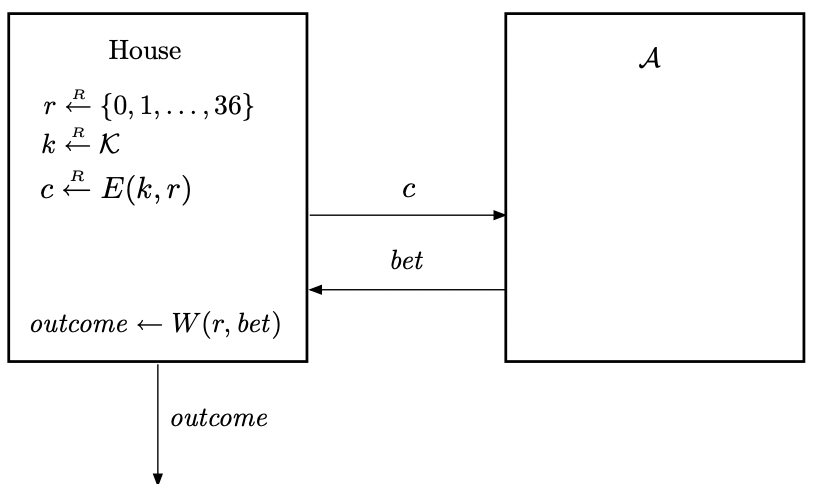
\includegraphics[width=0.6\linewidth]{figures/chapter2/fig2.png}
  \caption{网络轮盘赌}
  \label{fig:2-2}
\end{figure}

\begin{theorem}
如果 $\mathcal{E}$ 是语义安全的,那么对于每个有效玩家 $\mathcal{A}$,${\rm IR\mathsf{adv}}[\mathcal{A}]$ 的值都可忽略不计。
\end{theorem}

\begin{proof}
如我们在 \ref{subsec:2-2-3} 节所做的那样,我们仍然通过安全规约来证明这一点。更具体地说,我们将证明,对于每个玩家 $\mathcal{A}$,都存在一个语义安全对手 $\mathcal{B}$,使得 $\mathcal{B}$ 是 $\mathcal{A}$ 的一个基本包装器,并且:
\begin{equation}\label{eq:2-7}
{\rm IR\mathsf{adv}}[A]={\rm SS\mathsf{adv}}[\mathcal{B},\mathcal{E}]
\end{equation}

因此,如果存在一个优势不可忽略不计的有效玩家 $\mathcal{A}$,我们就能够得到一个有效的语义安全对手 $\mathcal{B}$,它可以打破 $\mathcal{E}$ 的语义安全性,而我们已经假设这是不可能的。因此,不存在这样的 $\mathcal{A}$。

为了分析我们的新对手 $\mathcal{B}$,我们先考虑一个``理想化"的互联网轮盘赌版本。在这个版本中,庄荷不公布实际的 $r$ 的加密,而是公布一个``假"值的加密,例如 $0$。图 \ref{fig:2-3} 展示了这个理想化的网络轮盘赌的逻辑。然而,请注意,在理想化版本的互联网轮盘赌中,庄荷仍然使用 $r$ 的实际值来决定游戏的结果。令 $p_0$ 为 $\mathcal{A}$ 在互联网轮盘赌中获胜的概率,$p_1$ 为 $\mathcal{A}$ 在理想化互联网轮盘赌中获胜的概率。

\begin{figure}
  \centering
  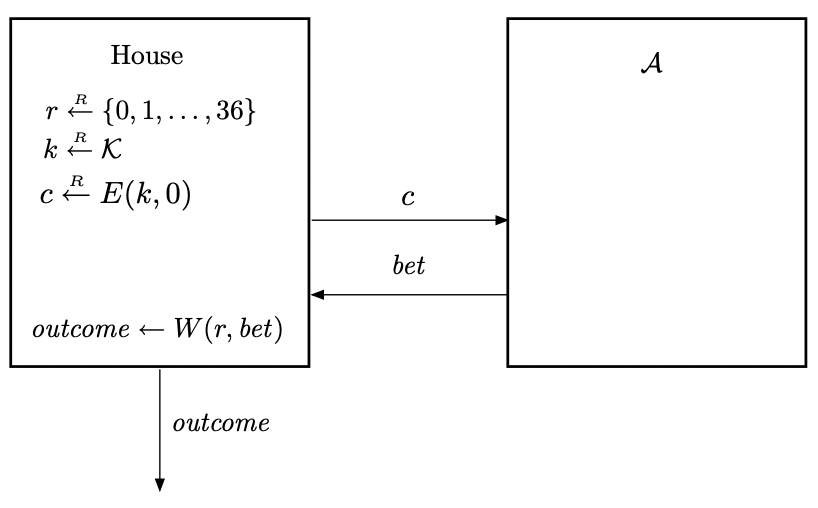
\includegraphics[width=0.6\linewidth]{figures/chapter2/fig3.png}
  \caption{网络轮盘赌的理想化版本}
  \label{fig:2-3}
\end{figure}

\begin{figure}
  \centering
  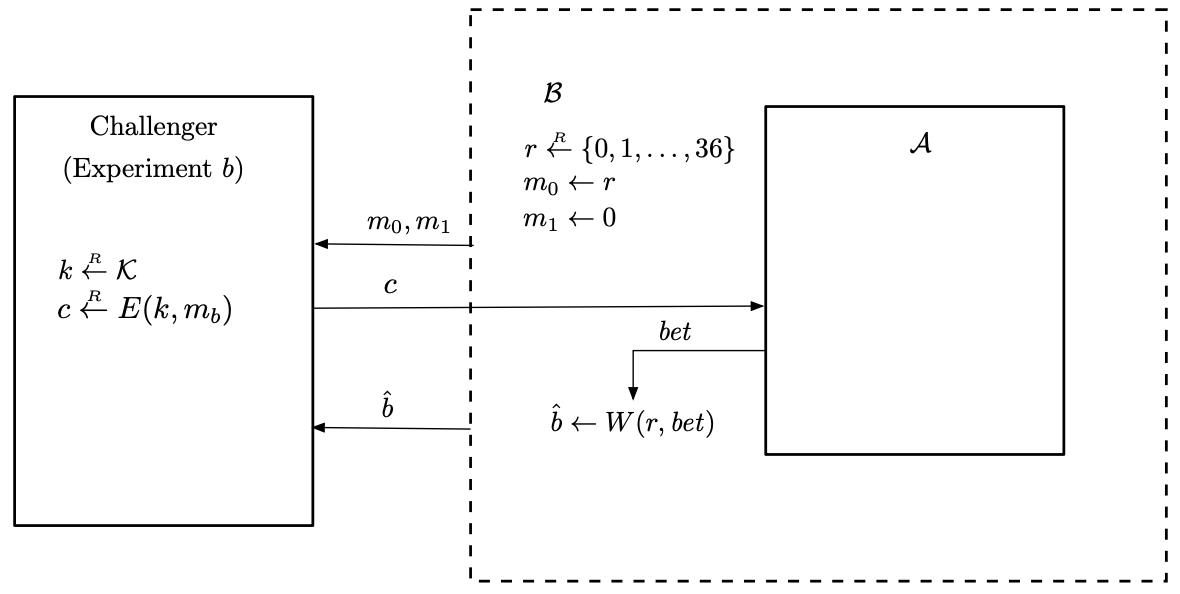
\includegraphics[width=0.85\linewidth]{figures/chapter2/fig4.png}
  \caption{攻击游戏 \ref{game:2-1} 中的语义安全对手 $\mathcal{B}$}
  \label{fig:2-4}
\end{figure}

我们的对手 $\mathcal{B}$ 被设计为在攻击游戏 \ref{game:2-1} 中进行游戏。因此,如果令 $\hat b$ 表示 $\mathcal{B}$ 在该游戏中的输出,我们有:
\begin{itemize}
	\item 如果 $\mathcal{B}$ 被置于实验 $0$ 中,那么有 $\Pr[\hat b=1]=p_0$;
	\item 如果 $\mathcal{B}$ 被置于实验 $1$ 中,那么有 $\Pr[\hat b=1]=p_1$。
\end{itemize}
图 \ref{fig:2-4} 展示了对手 $\mathcal{B}$ 的运行逻辑。通过构造可以看出,$\mathcal{B}$ 满足上面所声称的属性,特别是:
\begin{equation}\label{eq:2-8}
{\rm SS\mathsf{adv}}[\mathcal{B},\mathcal{E}]=|p_1-p_0|
\end{equation}

现在,考虑 $\mathcal{A}$ 在理想化互联网轮盘赌中获胜的概率 $p_1$。不管 $\mathcal{A}$ 的策略有多高明,他获胜的概率始终是 $18/37$,因为在这个理想化互联网轮盘赌中,\emph{赌注}的值是由 $c$ 计算出来的,而 $c$ 在统计上与 $r$ 的值毫无关系。因此:
\begin{equation}\label{eq:2-9}
{\rm IR\mathsf{adv}}[A]=|p_1-p_0|
\end{equation}

结合式 \ref{eq:2-8} 和式 \ref{eq:2-9},我们就能得到式 \ref{eq:2-7}。
\end{proof}

我们之后会反复使用这里用来分析互联网轮盘赌的方法。其基本思想是用一个理想化的系统组件替换原来的组件,然后分析这个新的、理想化版本的系统行为。

从上述例子中得到的另一个教训是,在推理一个系统的安全性时,我们将什么视为``对手",取决于我们想要做什么。在上面的分析中,我们用几个组件拼凑了一个新的对手 $\mathcal{B}$:其中一个组件是原来的对手 $\mathcal{A}$,而其他组件则是从系统的其他部分(在这个例子中是``庄荷"的算法)搜刮来的。这在我们全书的安全分析中会非常典型。直观地说,如果我们想象一个系统图,在安全分析的不同点上,我们将在系统的不同组件周围画一个圆圈,以确定我们在分析那个点时的``对手"。

\subsection{比特猜测:语义安全性的另一种表征}\label{subsec:2-2-5}

\ref{subsec:2-2-4} 小节中的例子很典型,它说明人们可以使用语义安全的定义来分析使用语义安全密码的较大系统的安全属性。然而,语义安全还有另一种更便于使用的表征,当我们试图证明一个给定的密码满足该定义时,它往往更方便使用。在这个替代性的表述中,我们定义一个新的攻击游戏。对手所扮演的角色与之前完全相同。然而,我们现在不再进行两个不同的实验,而是只有一个单一的实验。在这个\textbf{比特猜测版本(bit-guessing version)}的攻击游戏中,挑战者随机选择一个比特 $b\in\{0,1\}$并运行攻击游戏 \ref{game:2-1} 中的实验 $b$;对手的目标是以明显优于 ${1}/{2}$ 的概率猜中比特 $b$。下面是该攻击游戏的详细情况。

\begin{game}[语义安全性:比特猜测版本]\label{game:2-4}
给定一个定义在 $(\mathcal{K},\mathcal{M},\mathcal{C})$ 上的密码 $\mathcal{E}=(E,D)$,对于一个给定对手 $\mathcal{A}$,攻击游戏按如下方式运行:
\begin{itemize}
	\item 对手 $\mathcal{A}$ 计算相同长度的 $m_0, m_1\in\mathcal{M}$,并将它们发送给挑战者。
	\item 挑战者计算 $b\overset{\rm R}\leftarrow\{0,1\}$,$k\overset{\rm R}\leftarrow\mathcal{K}$,$c\overset{\rm R}\leftarrow E(k,m_b)$,并将 $c$ 发送给对手。
	\item 对手输出一个比特 $\hat b\in\{0,1\}$。
\end{itemize}

如果 $\hat b=b$,我们就称 $\mathcal{A}$ \textbf{赢得}这个游戏。
\end{game}

\begin{figure}
  \centering
  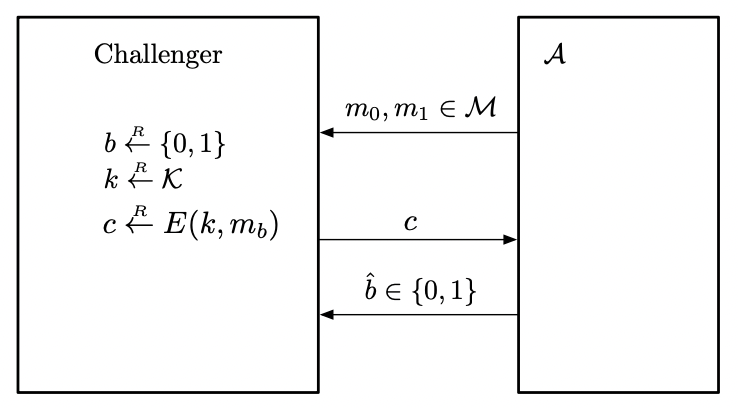
\includegraphics[width=0.5\linewidth]{figures/chapter2/fig5.png}
  \caption{攻击游戏 \ref{game:2-4}}
  \label{fig:2-5}
\end{figure}

图 \ref{fig:2-5} 展示了攻击游戏 \ref{game:2-4}。请注意,在这个游戏中,$\mathcal{A}$ 赢得游戏的事件是由 $b$ 与 $k$ 的随机选择、加密算法的随机选择(如果有的话)和对手的随机选择(如果有的话)共同构成的概率空间所定义的。

当然,任何对手都能以 ${1}/{2}$ 的概率赢得游戏,只需要完全忽略 $c$ 并随机选择 $\hat b$(或者说总是选择$\hat b=0$或总是选择$\hat b =1$)。我们感兴趣的是,对手能比随机猜测好多少。如果用 $W$ 表示对手赢得上述攻击游戏的比特猜测版本的事件,那么我们感兴趣的是 $|\Pr[W]-{1}/{2}|$ 的值,我们用 ${\rm SS\mathsf{adv}}^∗[\mathcal{A},\mathcal{E}]$ 表示该值。于是,我们有:

\begin{theorem}\label{theo:2-10}
对于每个密码 $\mathcal{E}$ 和每个对手 $\mathcal{A}$,我们都有:
\begin{equation}\label{eq:2-10}
{\rm SS\mathsf{adv}}[\mathcal{B},\mathcal{E}]= 2\cdot{\rm SS\mathsf{adv}}^∗[\mathcal{A},\mathcal{E}]
\end{equation}
\end{theorem}

\begin{proof}
这只是一个简单的计算。令 $p_0$ 是对手在攻击游戏 \ref{game:2-1} 的实验 $0$ 中输出 $1$ 的概率,$p_1$ 是对手在攻击游戏 \ref{game:2-1} 的实验 $1$ 中输出 $1$ 的概率。

现在考虑攻击游戏 \ref{game:2-4}。从现在开始,所有的事件和概率都是关于这个游戏的。如果我们以 $b=0$ 这一事件为条件,那么在这个条件概率空间中,挑战者和对手的所有其他随机选择的分布方式与攻击游戏 \ref{game:2-1} 的实验 $0$ 中的相应数值应该完全相同。因此,如果 $\hat b$ 是攻击游戏 \ref{game:2-4} 中对手的输出,则有:
$$
\Pr[\hat b=1\,|\,b=0]=p_0
$$
通过一个类似的论证,我们还可以得到:
$$
\Pr[\hat b=1\,|\,b=1]=p_1
$$
因此,我们有:
$$
\begin{aligned}
\Pr[\hat b=b]
&=\Pr[\hat b=b\,|\,b=0]\cdot\Pr[b=0]+\Pr[\hat b=b\,|\,b=1]\cdot\Pr[b=1]\\
&=\Pr[\hat b=0\,|\,b=0]\cdot \frac{1}{2}+\Pr[\hat b=b\,|\,b=1]\cdot\frac{1}{2}\\
& =\frac{1}{2}(1-\Pr[\hat b=1\,|\,b=0]+\Pr[\hat b=1\,|\,b=1])\\
& =\frac{1}{2}(1-p_0+p_1)
\end{aligned}
$$
因此:
$$
{\rm SS\mathsf{adv}}^∗[\mathcal{A},\mathcal{E}]=|\Pr[\hat b=b]-\frac{1}{2}|=\frac{1}{2}|p_1-p_0|=\frac{1}{2}\cdot{\rm SS\mathsf{adv}}[\mathcal{B},\mathcal{E}]
$$
这就证明了该定理。
\end{proof}

就像把 ${\rm SS\mathsf{adv}}[\mathcal{A},\mathcal{E}]$ 称为 $\mathcal{A}$ 的``语义安全优势"一样,我们将把 ${\rm SS\mathsf{adv}}^∗[\mathcal{A},\mathcal{E}]$ 称为 $\mathcal{A}$ 的``比特猜测语义安全优势"。

\subsubsection{一种推广}

事实证明,上面的情况是相当普遍的。虽然我们在本章中不需要它,但为了将来参考,我们在此指出如何推广上述情况到更一般的场景。我们可能会遇到一些情况,对于一些密码学系统(称为``$\mathcal{S}$"),其中的一些特定的安全属性(称为``$X$")可以用涉及两个实验(实验$0$和实验$1$)的攻击游戏来定义,其中对手 $\mathcal{A}$ 的协议在两个实验中是相同的,而挑战者的协议则是不同的。对于 $b=0,1$,我们定义 $W_b$ 为 $\mathcal{A}$ 在实验 $b$ 中输出为 $1$ 的事件,我们还定义:
$$
{\rm X\mathsf{adv}}[\mathcal{A},\mathcal{S}]:=|\Pr[W_0] -\Pr[W_1]|
$$
是 $\mathcal{A}$ 的 ``$X$ 优势"。就像上面一样,我们总是可以定义该攻击游戏的比特猜测版本,此时,挑战者随机选择一个 $b\in\{0,1\}$,然后运行实验 $b$ 作为它的协议。如果令 $W$ 是对手 $\mathcal{A}$ 的输出为 $b$ 的事件,那么我们定义:
$$
{\rm X\mathsf{adv}}^*[\mathcal{A},\mathcal{S}]:=|\Pr[W]-{1}/{2}|
$$
是 $\mathcal{A}$ 的``比特猜测$X$优势"。

使用与定理 \ref{theo:2-10} 的证明完全相同的计算方法,我们有:
\begin{equation}\label{eq:2-11}
{\rm X\mathsf{adv}}[\mathcal{A},\mathcal{S}]=2\cdot{\rm X\mathsf{adv}}^*[\mathcal{A},\mathcal{S}]
\end{equation}